% answers.tex —— 1977 年·上海卷·理科 · 参考答案与详细解析片段
% 由 tools/generate_projects.py 依来源总账自 1977/1977_数学真题_上海理_试题.md + 1977/1977_数学真题_上海理_解析正文.md + 1977/1977_数学真题_上海理_答案要点.md 生成，勿手改（改源 MD 后重跑）


\begin{gktip}
下列推导依据固定源 A3 单页题面独立完成，未使用官方答案页；因此解析与答案要点均不声称为官方标准答案。第 9、10 题保留为原卷附加题，正式题量仍为 8 题。
\end{gktip}

\begin{answer}
\gksolhead{1}{}

\textbf{题目}：

\Needspace{5\baselineskip}
（1） 化简：

\nopagebreak[4]
\[
\left(\frac{a}{a+b}-\frac{a^2}{a^2+2ab+b^2}\right)\div\left(\frac{a}{a+b}-\frac{a^2}{a^2-b^2}\right).
\]

\Needspace{5\baselineskip}
（2） 计算：

\nopagebreak[4]
\[
\frac12\lg25+\lg2-\lg\sqrt{0.1}-\log_2 9\times\log_3 2.
\]

\Needspace{5\baselineskip}
（3） $\sqrt{-1}=i$，验算 $i$ 是否方程

\nopagebreak[4]
\[
2x^4+3x^3-3x^2+3x-5=0
\]

的解。

\Needspace{5\baselineskip}
（4） 求证：

\nopagebreak[4]
\[
\frac{\sin\left(\frac\pi4+\theta\right)}{\sin\left(\frac\pi4-\theta\right)}+\frac{\cos\left(\frac\pi4+\theta\right)}{\cos\left(\frac\pi4-\theta\right)}=\frac{2}{\cos2\theta}.
\]

\Needspace{4\baselineskip}
\textbf{解析}

\gksubpart{（1）}

\Needspace{5\baselineskip}
在原式有意义的条件下，$a+b\ne0$、$a-b\ne0$ 且 $ab\ne0$。先分别化简两个括号：

\nopagebreak[4]
\[
\frac{a}{a+b}-\frac{a^2}{(a+b)^2}=\frac{ab}{(a+b)^2},
\]

\nopagebreak[4]
\[
\frac{a}{a+b}-\frac{a^2}{(a-b)(a+b)}
=-\frac{ab}{(a-b)(a+b)}.
\]

\Needspace{5\baselineskip}
所以原式为

\nopagebreak[4]
\[
\frac{ab}{(a+b)^2}\div\left(-\frac{ab}{(a-b)(a+b)}\right)
=-\frac{a-b}{a+b}=\frac{b-a}{a+b}.
\]

\gksubpart{（2）}

\nopagebreak[4]
\[
\frac12\lg25=\lg5,
\qquad
\lg\sqrt{0.1}=\frac12\lg10^{-1}=-\frac12.
\]

\Needspace{5\baselineskip}
又因为

\nopagebreak[4]
\[
\log_2 9\times\log_3 2
=2\log_2 3\times\frac1{\log_2 3}=2,
\]

\Needspace{5\baselineskip}
故原式为

\nopagebreak[4]
\[
\lg5+\lg2-\left(-\frac12\right)-2
=1+\frac12-2=-\frac12.
\]

\gksubpart{（3）}

\nopagebreak[4]
\[
i^2=-1,\qquad i^3=-i,\qquad i^4=1.
\]

\Needspace{5\baselineskip}
代入方程左端：

\nopagebreak[4]
\[
2i^4+3i^3-3i^2+3i-5
=2-3i+3+3i-5=0.
\]

所以 $i$ 是该方程的解。

\gksubpart{（4）}

\Needspace{5\baselineskip}
令 $c=\cos\theta$、$s=\sin\theta$。由和差角公式，

\nopagebreak[4]
\[
\sin\left(\frac\pi4+\theta\right)=\frac{c+s}{\sqrt2},
\quad
\sin\left(\frac\pi4-\theta\right)=\frac{c-s}{\sqrt2},
\]

\nopagebreak[4]
\[
\cos\left(\frac\pi4+\theta\right)=\frac{c-s}{\sqrt2},
\quad
\cos\left(\frac\pi4-\theta\right)=\frac{c+s}{\sqrt2}.
\]

\Needspace{5\baselineskip}
因此左端为

\nopagebreak[4]
\[
\frac{c+s}{c-s}+\frac{c-s}{c+s}
=\frac{(c+s)^2+(c-s)^2}{c^2-s^2}
=\frac{2(c^2+s^2)}{\cos2\theta}
=\frac2{\cos2\theta}.
\]

在原式有意义的定义域内，所用分母均不为零，等式成立。

\gkanswer{答案（1）：$\dfrac{b-a}{a+b}$。}

\gkanswer{答案（2）：$-\dfrac12$。}

\gkanswer{答案（3）：$i$ 是该方程的解。}

\gkanswer{答案（4）：见解析版}

\end{answer}
\begin{answer}
\gksolhead{2}{}

\textbf{题目}：

在 $\triangle ABC$ 中，$\angle C$ 的平分线交 $AB$ 于 $D$，过 $D$ 作 $BC$ 的平行线交 $AC$ 于 $E$，已知 $BC=a$，$AC=b$，求 $DE$ 的长。
\nopagebreak[4]
\begin{center}% 1977 年上海卷理科第 2 题：角平分线与平行线
\begin{tikzpicture}[scale=0.9]
  \coordinate (A) at (0,0);
  \coordinate (C) at (5,0);
  \coordinate (B) at (2.25,3.15);
  \coordinate (D) at ($(A)!0.43!(B)$);
  \coordinate (E) at ($(A)!0.43!(C)$);
  \draw[thick] (A)--(B)--(C)--cycle;
  \draw[thick] (D)--(C);
  \draw[thick] (D)--(E);
  \fill (A) circle (1.2pt) node[below left] {$A$};
  \fill (B) circle (1.2pt) node[above] {$B$};
  \fill (C) circle (1.2pt) node[below right] {$C$};
  \fill (D) circle (1.2pt) node[left] {$D$};
  \fill (E) circle (1.2pt) node[below] {$E$};
\end{tikzpicture}
\end{center}
\nopagebreak[4]
\Needspace{4\baselineskip}
\textbf{解析}

\Needspace{5\baselineskip}
由 $CD$ 是 $\angle C$ 的平分线，角平分线定理给出

\nopagebreak[4]
\[
\frac{AD}{DB}=\frac{AC}{CB}=\frac ba,
\qquad
\frac{AD}{AB}=\frac{b}{a+b}.
\]

\Needspace{5\baselineskip}
又因为 $DE\parallel BC$，所以 $\triangle ADE\sim\triangle ABC$，从而

\nopagebreak[4]
\[
\frac{DE}{BC}=\frac{AD}{AB}=\frac{b}{a+b}.
\]

\Needspace{5\baselineskip}
代入 $BC=a$，得到

\nopagebreak[4]
\[
DE=\frac{ab}{a+b}.
\]

\gkanswer{答案：$DE=\dfrac{ab}{a+b}$。}

\end{answer}
\begin{answer}
\gksolhead{3}{}

\textbf{题目}：

已知圆 $A$ 的直径为 $2\sqrt3$，圆 $B$ 的直径为 $4-2\sqrt3$，圆 $C$ 的直径为 $2$，圆 $A$ 与圆 $B$ 外切，圆 $A$ 又与圆 $C$ 外切，$\angle A=60^\circ$，求 $BC$ 及 $\angle C$。

\Needspace{4\baselineskip}
\textbf{解析}

\Needspace{5\baselineskip}
按题中“圆 $A$、圆 $B$、圆 $C$”的通常记号，将 $A\text{、}B\text{、}C$ 视为三个圆的圆心。三个圆的半径分别为

\nopagebreak[4]
\[
r_A=\sqrt3,\qquad r_B=2-\sqrt3,\qquad r_C=1.
\]

\Needspace{5\baselineskip}
由两圆外切时圆心距等于半径和，得

\nopagebreak[4]
\[
AB=r_A+r_B=2,
\qquad AC=r_A+r_C=1+\sqrt3.
\]

\Needspace{5\baselineskip}
在圆心三角形 $ABC$ 中，$\angle A=60^\circ$。由余弦定理，

\nopagebreak[4]
\[
\begin{aligned}
BC^2
&=AB^2+AC^2-2\,AB\cdot AC\cos60^\circ\\
&=4+(1+\sqrt3)^2-2(1+\sqrt3)=6.
\end{aligned}
\]

\Needspace{5\baselineskip}
所以 $BC=\sqrt6$。再由余弦定理求 $C$ 角：

\nopagebreak[4]
\[
\cos C
=\frac{AC^2+BC^2-AB^2}{2\,AC\cdot BC}
=\frac1{\sqrt2}.
\]

故 $\angle C=45^\circ$。

\gkanswer{答案：$BC=\sqrt6$，$\angle C=45^\circ$。}

\end{answer}
\begin{answer}
\gksolhead{4}{}

\textbf{题目}：

正六棱锥 $V-ABCDEF$ 的高为 $2\ \mathrm{cm}$，底面边长为 $2\ \mathrm{cm}$。

（1） 按 $1:1$ 画出它的二视图；

（2） 求其侧面积；

（3） 求它的侧棱和底面的夹角。

\Needspace{4\baselineskip}
\textbf{解析}

\gksubpart{（1）}

题面没有限定主视方向；下面给出一套按 $1:1$ 尺寸、采用“主视图+俯视图”的二视图方案，图中长度单位为 cm。

俯视图是边长 $2$ cm 的正六边形，顶点 $V$ 在底面中心 $O$ 的投影为 $V'$；取主视方向经过一对相对顶点，则主视图是底边 $4$ cm、高 $2$ cm 的等腰三角形。实、虚线布局会随主视方向旋转，但几何尺寸不变。
\nopagebreak[4]
\begin{center}% 1977 年上海卷理科第 4 题：正六棱锥的一套二视图（按 1:1 尺寸）
\begin{tikzpicture}[scale=0.72]
  \node at (2.1,4.15) {俯视图};
  \coordinate (O) at (2.1,2.95);
  \draw[thick] (4.1,2.95)--(3.1,4.68)--(1.1,4.68)--(0.1,2.95)--(1.1,1.22)--(3.1,1.22)--cycle;
  \fill (O) circle (1.2pt) node[below right] {$V'$};
  \draw[dashed] (O)--(4.1,2.95) (O)--(3.1,4.68) (O)--(1.1,4.68)
    (O)--(0.1,2.95) (O)--(1.1,1.22) (O)--(3.1,1.22);
  \node at (2.1,0.35) {主视图};
  \draw[thick] (0.35,-1.65)--(3.85,-1.65)--(2.1,0.35)--cycle;
  \draw[<->] (0.35,-1.95)--(3.85,-1.95) node[midway,below] {$4\ \mathrm{cm}$};
  \draw[<->] (4.15,-1.65)--(4.15,0.35) node[midway,right] {$2\ \mathrm{cm}$};
  \node[below] at (2.1,1.22) {底面边长 $2\ \mathrm{cm}$};
\end{tikzpicture}
\end{center}
\nopagebreak[4]
\gksubpart{（2）}

\Needspace{5\baselineskip}
设底面一边的中点为 $M$，底面中心为 $O$。正六边形边长为 $2$，所以

\nopagebreak[4]
\[
OM=\frac{2\sqrt3}{2}=\sqrt3.
\]

\Needspace{5\baselineskip}
正棱锥高 $VO=2$，故侧面三角形的斜高为

\nopagebreak[4]
\[
VM=\sqrt{VO^2+OM^2}=\sqrt{2^2+(\sqrt3)^2}=\sqrt7.
\]

\Needspace{5\baselineskip}
底面周长为 $6\times2=12$ cm，侧面积为

\nopagebreak[4]
\[
S_{\text{\text{侧}}}=6\cdot\frac12\cdot2\cdot\sqrt7=6\sqrt7\ \mathrm{cm^2}.
\]

\gksubpart{（3）}

\Needspace{5\baselineskip}
正六边形的外接圆半径等于边长，故 $OA=2$。在直角三角形 $VOA$ 中，侧棱 $VA$ 在底面内的正投影为 $OA$。若侧棱与底面的夹角为 $\varphi$，则

\nopagebreak[4]
\[
\tan\varphi=\frac{VO}{OA}=1.
\]

所以 $\varphi=45^\circ$。

\gkanswer{答案（1）：见解析版}

\gkanswer{答案（2）：$6\sqrt7\ \mathrm{cm^2}$。}

\gkanswer{答案（3）：$45^\circ$。}

\end{answer}
\begin{answer}
\gksolhead{5}{}

\textbf{题目}：

\Needspace{5\baselineskip}
解不等式：

\nopagebreak[4]
\[
\begin{cases}
16-x^2\geqslant0,\\
x^2-x-6>0,
\end{cases}
\]

并在数轴上把它的解表示出来。

\Needspace{4\baselineskip}
\textbf{解析}

\Needspace{5\baselineskip}
第一式给出

\nopagebreak[4]
\[
16-x^2\geqslant0\Longleftrightarrow -4\leqslant x\leqslant4.
\]

\Needspace{5\baselineskip}
第二式因式分解为

\nopagebreak[4]
\[
x^2-x-6=(x-3)(x+2)>0,
\]

\Needspace{5\baselineskip}
所以 $x<-2$ 或 $x>3$。两组条件取交集，得到

\nopagebreak[4]
\[
x\in[-4,-2)\cup(3,4].
\]

在数轴上，$-4$、$4$ 取到，$-2$、$3$ 不取到：
\nopagebreak[4]
\begin{center}% Q5: the solution of 16-x^2 >= 0 and x^2-x-6 > 0.
% Exact endpoints: closed at -4,4; open at -2,3.
\begin{center}
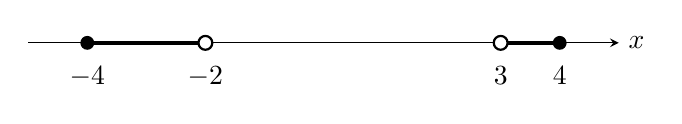
\begin{tikzpicture}[x=0.75cm,y=1cm,>=stealth]
  \draw[->] (-5,0)--(5,0) node[right] {$x$};
  \draw[very thick] (-4,0)--(-2,0) (3,0)--(4,0);
  \fill (-4,0) circle (2.5pt);
  \fill (4,0) circle (2.5pt);
  \draw[fill=white,thick] (-2,0) circle (2.5pt);
  \draw[fill=white,thick] (3,0) circle (2.5pt);
  \node[below=5pt] at (-4,0) {$-4$};
  \node[below=5pt] at (-2,0) {$-2$};
  \node[below=5pt] at (3,0) {$3$};
  \node[below=5pt] at (4,0) {$4$};
\end{tikzpicture}
\end{center}
\end{center}
\nopagebreak[4]
\gkanswer{答案：$[-4,-2)\cup(3,4]$。}

\end{answer}
\begin{answer}
\gksolhead{6}{}

\textbf{题目}：

已知两定点 $A(-4,0)$、$B(4,0)$，一动点 $P(x,y)$ 与两定点 $A\text{、}B$ 的连线 $PA\text{、}PB$ 的斜率的乘积为 $-\dfrac14$。求点 $P$ 的轨迹方程，并把它化为标准方程，指出是什么曲线。

\Needspace{4\baselineskip}
\textbf{解析}

\Needspace{5\baselineskip}
当 $x\ne-4,4$ 时，直线 $PA$、$PB$ 的斜率分别为

\nopagebreak[4]
\[
k_{PA}=\frac{y}{x+4},
\qquad
k_{PB}=\frac{y}{x-4}.
\]

\Needspace{5\baselineskip}
由题设

\nopagebreak[4]
\[
\frac{y^2}{(x+4)(x-4)}=-\frac14,
\]

\Needspace{5\baselineskip}
整理得

\nopagebreak[4]
\[
x^2+4y^2=16.
\]

\Needspace{5\baselineskip}
标准方程为

\nopagebreak[4]
\[
\frac{x^2}{16}+\frac{y^2}{4}=1.
\]

因此轨迹所在的曲线是以原点为中心、半轴长分别为 $4$ 和 $2$ 的椭圆。严格按斜率定义，$P=A(-4,0)$ 或 $P=B(4,0)$ 时相应斜率无定义，所以实际轨迹去掉这两个端点；通常将上述完整椭圆作为轨迹的标准方程。

\gkanswer{答案：$x^2+4y^2=16$，即 $\dfrac{x^2}{16}+\dfrac{y^2}{4}=1$，为椭圆；严格按斜率定义，$A(-4,0)$、$B(4,0)$ 两点不在实际轨迹中。}

\end{answer}
\begin{answer}
\gksolhead{7}{}

\textbf{题目}：

等腰梯形的周长为 $60$，底角为 $60^\circ$，问这梯形各边长为多少时，面积最大？
\nopagebreak[4]
\begin{center}% 1977 年上海卷理科第 7 题：等腰梯形
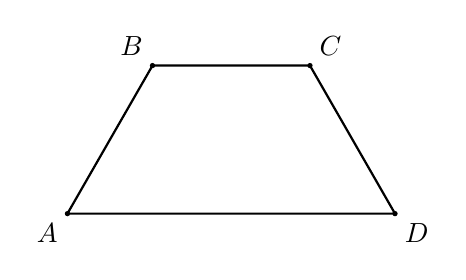
\begin{tikzpicture}[scale=0.8]
  \coordinate (A) at (0,0);
  \coordinate (D) at (5.2,0);
  \coordinate (B) at (1.35,2.35);
  \coordinate (C) at (3.85,2.35);
  \draw[thick] (A)--(B)--(C)--(D)--cycle;
  \fill (A) circle (1.2pt) node[below left] {$A$};
  \fill (B) circle (1.2pt) node[above left] {$B$};
  \fill (C) circle (1.2pt) node[above right] {$C$};
  \fill (D) circle (1.2pt) node[below right] {$D$};
\end{tikzpicture}
\end{center}
\nopagebreak[4]
\Needspace{4\baselineskip}
\textbf{解析}

\Needspace{5\baselineskip}
设两腰长为 $\ell$，下底 $AD=p$，上底 $BC=q$。由底角为 $60^\circ$，每条腰在水平方向的投影为 $\ell/2$，梯形高为

\nopagebreak[4]
\[
h=\ell\sin60^\circ=\frac{\sqrt3}{2}\ell,
\qquad p-q=\ell.
\]

\Needspace{5\baselineskip}
由周长条件 $p+q+2\ell=60$，得

\nopagebreak[4]
\[
q=\frac{60-3\ell}{2},\qquad p=\frac{60-\ell}{2}.
\]

\Needspace{5\baselineskip}
面积为

\nopagebreak[4]
\[
\begin{aligned}
S&=\frac{p+q}{2}h\\
&=\frac{60-2\ell}{2}\cdot\frac{\sqrt3}{2}\ell\\
&=\frac{\sqrt3}{2}\ell(30-\ell)\\
&=\frac{\sqrt3}{2}\left[225-(\ell-15)^2\right].
\end{aligned}
\]

\Needspace{5\baselineskip}
所以面积在 $\ell=15$ 时最大。此时

\nopagebreak[4]
\[
AB=CD=15,\qquad AD=\frac{45}{2},\qquad BC=\frac{15}{2},
\]

最大面积为 $225\sqrt3/2$。

\gkanswer{答案：两腰均为 $15$；下底 $\dfrac{45}{2}$，上底 $\dfrac{15}{2}$。此时面积最大，为 $\dfrac{225\sqrt3}{2}$。}

\end{answer}
\begin{answer}
\gksolhead{8}{}

\textbf{题目}：

\Needspace{5\baselineskip}
当 $k$ 为何值时，方程组

\nopagebreak[4]
\[
\left\{
\begin{aligned}
x-\sqrt{y-2}&=0 &&(1),\\
kx-y-2k-10&=0 &&(2)
\end{aligned}
\right.
\]

有两组相同的解？并求出它的解。

\begin{gktip}
\Needspace{0.25\textheight}
\textbf{附加题}
\end{gktip}

\textbf{附加题 9．} 如图所示，半圆 $O$ 的直径为 $2$，$A$ 为半圆直径的延长线上的一点，且 $OA=2$，$B$ 为半圆上任一点，以 $AB$ 为边作等边 $\triangle ABC$，问 $B$ 在什么地方时，四边形 $OACB$ 的面积最大？并求出这个面积的最大值。
\nopagebreak[4]
\begin{center}% 1977 年上海卷理科附加题：半圆与等边三角形
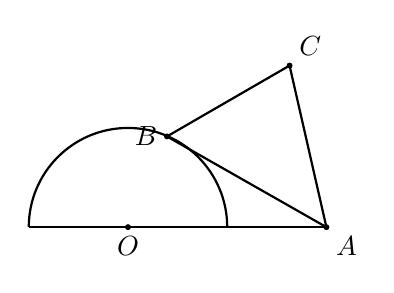
\begin{tikzpicture}[scale=0.9]
  \coordinate (O) at (0,0);
  \coordinate (L) at (-1.4,0);
  \coordinate (R) at (1.4,0);
  \coordinate (A) at (2.8,0);
  \coordinate (B) at (0.55,1.28);
  \coordinate (C) at (2.28,2.28);
  \draw[thick] (L) arc (180:0:1.4);
  \draw[thick] (L)--(A);
  \draw[thick] (B)--(A)--(C)--cycle;
  \fill (O) circle (1.2pt) node[below] {$O$};
  \fill (A) circle (1.2pt) node[below right] {$A$};
  \fill (B) circle (1.2pt) node[left] {$B$};
  \fill (C) circle (1.2pt) node[above right] {$C$};
  \draw[dashed] (O)--(A);
\end{tikzpicture}
\end{center}
\nopagebreak[4]
\textbf{附加题 10．} 已知曲线 $y=x^2-2x+3$ 与直线 $y=x+3$ 相交于点 $P(0,3)\text{、}Q(3,6)$ 两点。

\begin{itemize}
\item \textbf{（1）} 分别求出曲线在交点的切线的斜率；
\end{itemize}

\begin{itemize}
\item \textbf{（2）} 求出曲线与直线所围成的图形的面积。
\end{itemize}

\Needspace{4\baselineskip}
\textbf{解析}

\Needspace{5\baselineskip}
由第一个方程 $x-\sqrt{y-2}=0$，令

\nopagebreak[4]
\[
t=\sqrt{y-2}\geqslant0.
\]

\Needspace{5\baselineskip}
则 $x=t$、$y=t^2+2$。代入第二个方程，得到关于 $t$ 的二次方程

\nopagebreak[4]
\[
kt-(t^2+2)-2k-10=0
\Longleftrightarrow
t^2-kt+2k+12=0.
\]

\Needspace{5\baselineskip}
要有两组相同的解，判别式必须为零：

\nopagebreak[4]
\[
\Delta=k^2-4(2k+12)=k^2-8k-48=(k-12)(k+4)=0.
\]

\Needspace{5\baselineskip}
候选值为 $k=12$ 或 $k=-4$。当 $k=-4$ 时重根为 $t=-2$，不满足 $t\geqslant0$，舍去；当 $k=12$ 时 $t=6$，从而

\nopagebreak[4]
\[
x=6,\qquad y=6^2+2=38.
\]

故 $k=12$，相同的解为 $(6,38)$。

\gksubpart{附加题 9}

\Needspace{4\baselineskip}
\textbf{解析}

\Needspace{5\baselineskip}
半圆半径为 $1$。按图取

\nopagebreak[4]
\[
O=(0,0),\qquad A=(2,0),\qquad B=(\cos\theta,\sin\theta),
\quad 0\leqslant\theta\leqslant\pi.
\]

\Needspace{5\baselineskip}
取图示的等边三角形分支，使 $C$ 与 $O$ 位于直线 $AB$ 的两侧。先算

\nopagebreak[4]
\[
AB^2=(2-\cos\theta)^2+\sin^2\theta=5-4\cos\theta.
\]

\Needspace{5\baselineskip}
四边形 $OACB$ 的面积等于三角形 $OAB$ 与等边三角形 $ABC$ 的面积之和：

\nopagebreak[4]
\[
S_{OAB}=\frac12\cdot2\cdot\sin\theta=\sin\theta,
\]

\nopagebreak[4]
\[
S_{ABC}=\frac{\sqrt3}{4}AB^2=\frac{\sqrt3}{4}(5-4\cos\theta).
\]

\Needspace{5\baselineskip}
因此

\nopagebreak[4]
\[
\begin{aligned}
S_{OACB}
&=\frac{5\sqrt3}{4}+\sin\theta-\sqrt3\cos\theta\\
&=\frac{5\sqrt3}{4}+2\sin\left(\theta-\frac\pi3\right).
\end{aligned}
\]

\Needspace{5\baselineskip}
在 $0\leqslant\theta\leqslant\pi$ 内，最大值在 $\theta=5\pi/6$ 时取得。此时

\nopagebreak[4]
\[
B=\left(-\frac{\sqrt3}{2},\frac12\right),
\]

\Needspace{5\baselineskip}
且

\nopagebreak[4]
\[
S_{\max}=2+\frac{5\sqrt3}{4}.
\]

\gksubpart{附加题 10}

\Needspace{4\baselineskip}
\textbf{解析}

\Needspace{5\baselineskip}
曲线函数为 $y=x^2-2x+3$，故

\nopagebreak[4]
\[
y'=2x-2.
\]

\Needspace{5\baselineskip}
在 $P(0,3)$、$Q(3,6)$ 处的切线斜率分别为

\nopagebreak[4]
\[
k_P=-2,\qquad k_Q=4.
\]

\Needspace{5\baselineskip}
在 $0\leqslant x\leqslant3$ 上，直线在曲线上方，因为

\nopagebreak[4]
\[
(x+3)-(x^2-2x+3)=3x-x^2=x(3-x)\geqslant0.
\]

\Needspace{5\baselineskip}
所围图形面积为

\nopagebreak[4]
\[
\begin{aligned}
S&=\int_0^3\left[(x+3)-(x^2-2x+3)\right]\,\mathrm dx\\
&=\int_0^3(3x-x^2)\,\mathrm dx\\
&=\left[\frac32x^2-\frac13x^3\right]_0^3=\frac92.
\end{aligned}
\]

\gkanswer{答案：$k=12$，方程组的相同解为 $(x,y)=(6,38)$。}

\end{answer}